\title{Networking and System Security \\ Assignment 1}
\author{David van Erkelens (10264019) \\ Department of Computer Science \\ University of Amsterdam}
\date{\today}
\documentclass[12pt]{article}
\usepackage{graphicx}
\usepackage{color}
\begin{document}
\maketitle
\section{Task 1}
\begin{enumerate}
    \item The IP-address of \emph{ss64.com} is 216.92.29.160. \\
        The IP-adress of the sending computer is 145.18.214.201.
    \item There are 8 GET-requests to \emph{ss64.com} \\
        The filter used to find this result is \verb|http.request && ip.addr == 216.92.29.160|
    \item
        \begin{itemize}
            \item Ethernet II
            \item Internet Protocol Version 4
            \item Transmission Control Protocol
            \item Hypertext Transfer Protocol
        \end{itemize}
    \item There are 8 HTTP OK responses.
\end{enumerate}
\clearpage
\section{Task 2}
\begin{enumerate}
    \setcounter{enumi}{4}
    \item 0.434445 seconds. \\
        Retreived by showing only the HTTP traffic to \emph{ss64.com} and setting the view to \verb|Time Since Last Displayed Package|. The used filter is \verb|ip.addr == 216.92.29.160 && http|
    \item Yes, the following images:
        \begin{itemize}
            \item /images/ss64.gif
            \item /images/bash-l.gif
            \item /images/syntax-r.gif
            \item /images/top-4.gif
            \item /images/roll-left.png
            \item /images/roll-right.png
        \end{itemize}
    \item The requests are included as first-request.txt and first-ok.txt. They are printed by right clicking the package and selecting print, then selecting the print to file option.
\end{enumerate}

\section{Task 3}
\begin{enumerate}
    \setcounter{enumi}{7}
    \item There are 77 IPv4 packages send between \emph{ss64.com} and the user, with a total of 38558 bytes. A notable fact is that the number of bytes send to the host is much less than the number of received bytes. This can be explained by that fact that requests are send, and files are returned.
    \clearpage
    \item The used filters and the colors in which they are displayed in the graph:
        \begin{enumerate}
            \item {\color{black}\verb|No filter added|}
            \item {\color{red}\verb|ip.addr == 216.92.29.160 && tcp|}
            \item {\color{green}\verb|ip.addr == 216.92.29.160 && http.request|}
            \item {\color{blue}\verb|ip.addr == 216.92.29.160 && http.response|}
        \end{enumerate}
    Resulting in the following graph: \\
    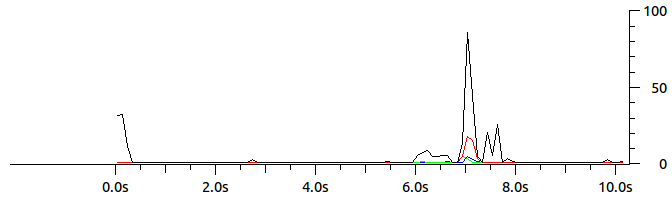
\includegraphics[width=\textwidth]{graph.png}
    When looking at the times shown at questions 2 and 4 and the times shown in the graph, it can be noticed that the graph is consistent with the earlier answers.
    \item There are two cleartext passwords in the packages:
        \begin{itemize}
            \item wrong!
            \item network
        \end{itemize}
    They are found by using the \verb|ip.addr = 128.119.245.12 && http.request| filter, and looking at the Authorization part of the package. When changing the filter to \verb|ip.addr = 128.119.245.12 && http|, it can be noted that "network" is the correct password, since this returns code 200 (OK) instead of code 401 (Authorization Required).
\end{enumerate}
\end {document}
